\documentclass{article}

% Packages
\usepackage{fancyhdr}
\usepackage{extramarks}
\usepackage{amsmath}
\usepackage{amsthm}
\usepackage{amsfonts}
\usepackage{tikz}
\usepackage[plain]{algorithm}
\usepackage{algpseudocode}
\usepackage{amssymb}
\usepackage{dsfont}
\usepackage{bbm}
\usepackage{geometry}
\usepackage{enumerate}
\usepackage{graphicx}

\usetikzlibrary{automata,positioning}

% Document Layout
\topmargin=-0.45in
\evensidemargin=0in
\oddsidemargin=0in
\textwidth=6.5in
\textheight=9.0in
\headsep=0.25in
\linespread{1.1}

% Page Style
\pagestyle{fancy}
\lhead{\hmwkAuthorName}
\chead{\hmwkClass:\ \hmwkTitle}
\rhead{Section \hmwkSection, \firstxmark}
\lfoot{\lastxmark}
\cfoot{\thepage}
\renewcommand\headrulewidth{0.4pt}
\renewcommand\footrulewidth{0.4pt}

% Paragraph Settings
\setlength\parindent{0pt}
\setlength{\parskip}{5pt}

% Section Management
\newcommand{\hmwkSection}{A} % Current section (A, B, or C) - update manually

% Problem Header Management
\newcommand{\enterProblemHeader}[1]{
  \nobreak\extramarks{}{Problem \arabic{#1} continued on next page\ldots}\nobreak{}
  \nobreak\extramarks{Problem \arabic{#1} (continued)}{Problem \arabic{#1} continued on next page\ldots}\nobreak{}
}

\newcommand{\exitProblemHeader}[1]{
  \nobreak\extramarks{Problem \arabic{#1} (continued)}{Problem \arabic{#1} continued on next page\ldots}\nobreak{}
  \stepcounter{#1}
  \nobreak\extramarks{Problem \arabic{#1}}{}\nobreak{}
}

% Counters
\setcounter{secnumdepth}{0}
\newcounter{partCounter}
\newcounter{homeworkProblemCounter}
\setcounter{homeworkProblemCounter}{1}
\nobreak\extramarks{Problem \arabic{homeworkProblemCounter}}{}\nobreak{}

% Homework Problem Environment
% Optional argument adjusts problem counter for non-sequential problems
\newenvironment{homeworkProblem}[1][-1]{
  \ifnum#1>0
    \setcounter{homeworkProblemCounter}{#1}
  \fi
  \section{Problem \arabic{homeworkProblemCounter}}
  \setcounter{partCounter}{1}
  \enterProblemHeader{homeworkProblemCounter}
}{
  \exitProblemHeader{homeworkProblemCounter}
}

% Assignment Details
\newcommand{\hmwkTitle}{Sheet\ \#1}
\newcommand{\hmwkDueDate}{Feb 9, 2026}
\newcommand{\hmwkClass}{C5.4 Networks}
\newcommand{\hmwkClassInstructor}{Professor R. Lambiotte}
\newcommand{\hmwkAuthorName}{\textbf{Ray Tsai}}

% Title Page
\title{
  \vspace{2in}
  \textmd{\textbf{\hmwkClass:\ \hmwkTitle}}\\
  \normalsize\vspace{0.1in}\small{Due\ on\ \hmwkDueDate\ at 12:00pm}\\
  \vspace{0.1in}\large{\textit{\hmwkClassInstructor}} \\
  \vspace{3in}
}

\author{\hmwkAuthorName}
\date{}

% Part Command
\renewcommand{\part}[1]{\textbf{\large Part \Alph{partCounter}}\stepcounter{partCounter}\\}

% Mathematical Commands
% Algorithms
\newcommand{\alg}[1]{\textsc{\bfseries \footnotesize #1}}

% Calculus
\newcommand{\deriv}[1]{\frac{\mathrm{d}}{\mathrm{d}x} (#1)}
\newcommand{\pderiv}[2]{\frac{\partial}{\partial #1} (#2)}
\newcommand{\dx}{\mathrm{d}x}

% Probability and Statistics
\newcommand{\Var}{\mathrm{Var}}
\newcommand{\Cov}{\mathrm{Cov}}
\newcommand{\Bias}{\mathrm{Bias}}
\newcommand*{\prob}{\mathbb{P}}
\newcommand*{\E}{\mathbb{E}}

% Number Sets
\newcommand*{\Z}{\mathbb{Z}}
\newcommand*{\Q}{\mathbb{Q}}
\newcommand*{\R}{\mathbb{R}}
\newcommand*{\C}{\mathbb{C}}
\newcommand*{\N}{\mathbb{N}}

\begin{document}

\maketitle
\pagebreak

\begin{homeworkProblem}
  \begin{enumerate}[(a)]
    \item Write down the total probability of drawing a graph $G$ with exactly $m$ edges from the ensemble $\mathcal{G}(N,p)$ and use it to find the mean value of edges $\langle m \rangle$.
    \begin{proof}
      Let $G \sim \mathcal{G}(N, p)$. Then
      \[
        \prob(e(G) = m) = \binom{\binom{N}{2}}{m}p^m(1 - p)^{\binom{N}{2} - m}.
      \]
      Note that $\prob(e(G) = m)$ follows a binomial distribution with parameter $p$ and $n = \binom{N}{2}$. Thus,
      \[
        \langle m \rangle = \binom{N}{2}p.
      \]
    \end{proof}

    \item Calculate the expected mean degree of an ER graph.
    \begin{proof}
      Let $d$ be the mean degree of $G \sim \mathcal{G}(N, p)$. By the handshake lemma,
      \[
        \langle d \rangle = \frac{2}{N}\langle m \rangle = (N - 1)p.
      \]
    \end{proof}

    \item Show, under an appropriate assumption (which you should state), that the degree distribution for an ER graph (in expectation over the ensemble) satisfies
    \begin{equation}
      p_{k} \sim e^{-c}\frac{c^{k}}{k!} \quad \text{as} \quad N \rightarrow \infty
    \end{equation}
    where $c = (N-1)p$.

    \begin{proof}
      Suppose $p = c/(N - 1)$ for some $c > 0$. Put $n = N - 1$. Then
      \begin{align*}
        p_k 
        &= \binom{n}{k}p^k(1 - p)^{n - k} \\
        &= \frac{n!}{k!(n - k)!}\left(\frac{c}{n}\right)^k\left(1 - \frac{c}{n}\right)^{n - k} \\
        &= \frac{c^k}{k!} \cdot \frac{n!}{(n - k)!} \cdot \left(\frac{1}{n}\right)^k\left(1 - \frac{c}{n}\right)^{n - k}.
      \end{align*}
      Note that
      \[
        \lim_{N \to \infty} \frac{n!}{(n - k)!n^k} = \lim_{N \to \infty} \left(1 - \frac{1}{n}\right) \left(1 - \frac{2}{n}\right) \cdots \left(1 - \frac{k - 1}{n}\right) = 1,
      \]
      so
      \[
        p_k \to \frac{c^k}{k!}\left(1 - \frac{c}{n}\right)^{n - k} = \frac{c^k}{k!} e^{-c},
      \]
      as $n \to \infty$.
    \end{proof}

    \newpage

    \item Calculate the global clustering coefficient $C$ of an ER graph (in expectation over the ensemble).
    \begin{proof}
      The global clustering coefficient is given by
      \[
        C = \frac{\binom{N}{3}p^3}{\binom{N}{3}p^2} = p,
      \]
      which is constant if $p$ is constant.
    \end{proof}

    \item Show that the diameter of an ER graph (again, in expectation over the ensemble) grows like $\ln N$ as $N \rightarrow \infty$.
    \begin{proof}
      Let $D$ be the expected diameter of $G \sim \mathcal{G}(N, p)$. Note that for $G$ to have diameter $D$, any vertex $v \in V(G)$ must reach all other vertices within $D$ steps of BFS. Put $c = (N - 1)p$. By (b), we are expected to reach $1 + c + c^2 + \cdots + c^{D - 1}$ vertices at step $D$. Thus we have
      \[
        1 + c + c^2 + \cdots + c^{D - 1} = \frac{1 - c^{D}}{1 - c} \approx N. 
      \]
      Solving for $D$, we get
      \[
        D \approx \frac{\log(1 + N(c - 1))}{\log c} = \Theta(\log N).
      \]
    \end{proof}
  \end{enumerate}
\end{homeworkProblem}

\newpage

% To change sections, use: \renewcommand{\hmwkSection}{B}
% Example: Uncomment the line below when you start Section B
\renewcommand{\hmwkSection}{B}

\begin{homeworkProblem}
  \begin{enumerate}[(a)]
    \item By means of numerical simulations, investigate the properties of the degree distribution of 3 variations of the BA model, where the probability to connect to a node is uniform, proportional to its degree, and proportional to the square of its degree, respectively. For simplicity consider the case when the new nodes enter the system with one single edge.
    
    How does the maximum degree in the graph evolve in time?
    
    How does the average distance between nodes evolve in time?

    Describe and interpret your findings.

    \begin{proof}[Solution]
      Here are the results of the numerical simulations:
      \begin{figure}[h]
        \centering
        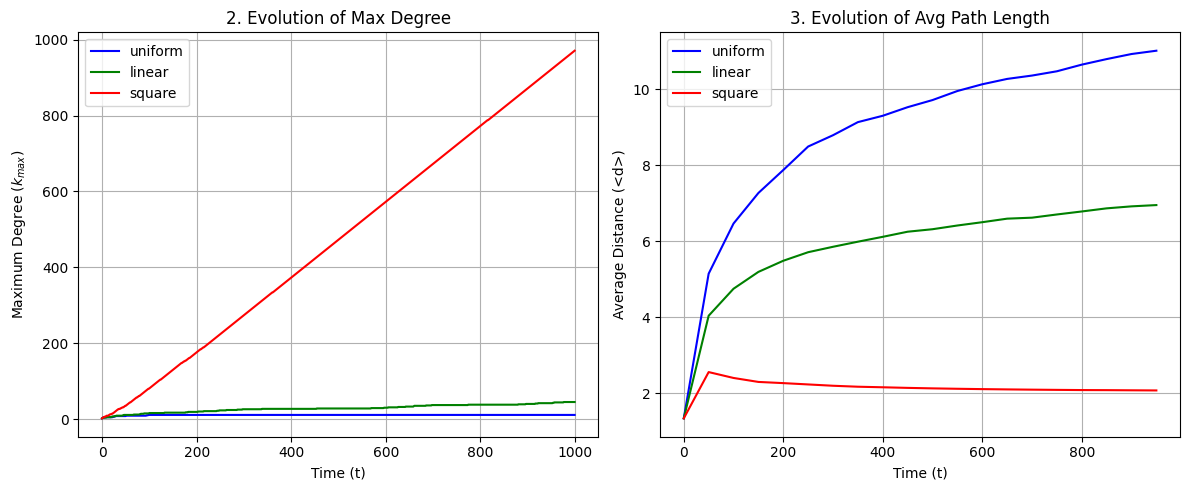
\includegraphics[width=0.9\textwidth]{images/2a.png}
      \end{figure}

      Notice that the maximum degree grows linearly in the square case. This is a natural consequence of the fact that the new node is heavily weighted towards connecting to the nodes with the highest degree. 
    \end{proof}

    \item Consider the model described in ``Structural transitions in densifying networks'', PRL 2016. The network grows by adding nodes sequentially. Each new node connects to a randomly chosen target node and, in addition, independently to each of the neighbours of the target with probability $p$.
    
    Derive an equation for the time evolution of the average number of links, and investigate its asymptotic behaviour. How would you characterise the regime when $p > \frac{1}{2}$?
    
    Derive a recursive relation for the stationary degree distribution and determine its tail in the sparse regime $p < \frac{1}{2}$.
\end{enumerate}
\end{homeworkProblem}

\end{document}